\section{mbeddr}


The mbeddr open-source project\footnote{ \url{http://mbeddr.com}} 
focuses on supporting embedded software
development. It introduces a set of of modular domain-specific extensions
to C and also supports other languages for addressing common problems 
in software development, \eg writing documentation with close 
integration to code or capturing requirements. mbeddr is build using 
JetBrains \ac{MPS} language 
workbench\footnote{ \url{https://www.jetbrains.com/mps/}}.
\fig{mbeddrArch} shows how mbeddr is organized into layers, with \ac{MPS} at
the bottom and custom language extensions on top.
\ac{MPS} supports the definition, 
composition and use of general purpose or domain-specific languages. 
To archive this \ac{MPS} uses a projectional editor, this means, even 
if the notation might look textual it is not represented as a sequence 
of characters, which are transformed into a \ac{AST} by parsing. 
In contrast user actions manipulate the \ac{AST} directly. The \ac{AST} 
is then rendered to the user according to editor specifications/projection
rules. These rules are not limited to textual notations, for example can tabular
or mathematical notations can be used if appropriated. Since no parsing ambiguities 
can occur a wide range of languages extension can be supported.

\begin{figure}[h]
  \vspace{-2mm}
  \centering
    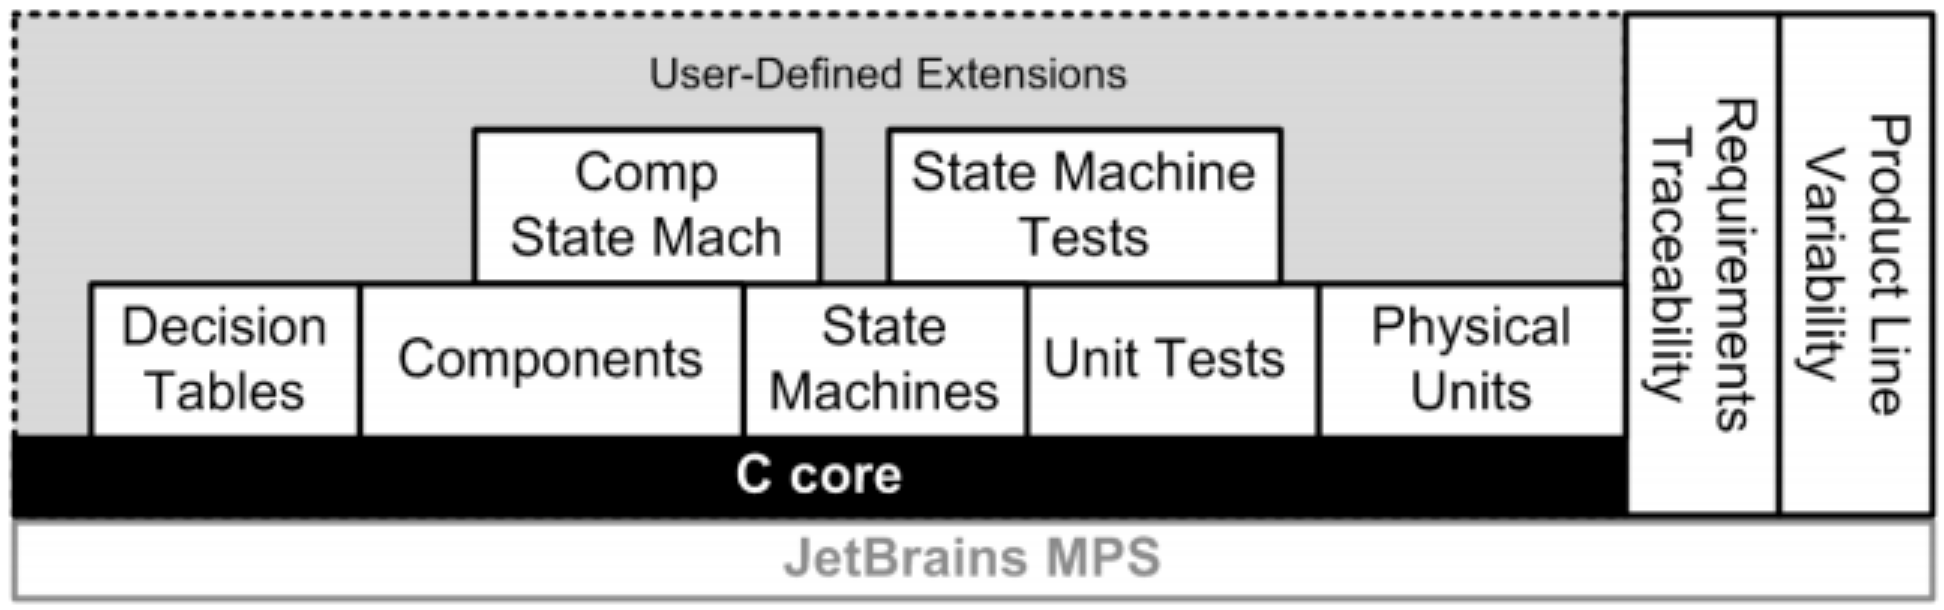
\includegraphics[width=8.5cm]{./figures/mbeddArch.png} 
    \vspace{-2mm}
    \caption{mbeddr language architecture~\cite{Voelter:2012:MEC:2384716.2384767}}
  \label{mbeddrArch}
  \vspace{-2mm}
\end{figure}


\subsection{Languages}
\label{languageImplementation}
mbeddr includes a extensible C99 implementation. In addition to plain C 
mbeddr also include a set of predefined extension on top of C. These 
extension include test cases, state machines, components and physical units. 
In \ac{MPS} languages are separated into modular aspects. The major aspects 
of a language are:  

\parhead{Structure:} Definition of the \ac{AST} of the language.

\parhead{Editor:} Projection rules how the \ac{AST} is presented to the user and how the user interacts with the program.

\parhead{Type System/Contraints:} Static semantics of the language.
 
\parhead{Generator:} Dynamic semantics of the language, transforms the model into executable code.

\subsection{Unit Test Language Extension}

This section shows the implementation of a minimal unit test language for
writing test cases with mbeddr. \lst{lst:generatedUT} shows a code
snippet.

\noindent 
\begin{minipage}[t]{120pt} 
\begin{lstlisting}[language=reducedMbeddr]
int32 main(int32 argc,
		string[] argv) {
   return $\colorbox{g1}{test[}$$\colorbox{g6}{forTest}$$\colorbox{g1}{]}$;
}
$\colorbox{white}{\hspace{2mm}{\color{white}\_fails;}}$
$\colorbox{white}{\hspace{2mm}{\color{white}blockexpr\_2();}}$
$\colorbox{white}{\hspace{2mm}{\color{white}\}}}$
$\colorbox{white}{\hspace{2mm}{\color{white}\}}}$
$\colorbox{white}{\hspace{2mm}{\color{white}int32\_t bp\_2() \{}}$ 
$\colorbox{white}{\hspace{2mm}{\color{white}i32\_t \_fails = 0;}}$		



$\colorbox{g7}{testcase forTest \{}$ 
$\colorbox{white}{\hspace{2mm}{\color{white}|}}$
   int32 sum = 0;
   int32[] nums = {1, 2, 3};
   for(int32_t i=0;i<3;i++){
     sum += nums[i];
   }
$\colorbox{g3}{\hspace{2.5mm}assert-equals sum == 3;}$
$\colorbox{white}{{\color{white}\_fails++;}}$
$\colorbox{white}{\hspace{5mm}{\color{white}pf("fal:\%d!3");}}$
$\colorbox{white}{\hspace{2mm}{\color{white}\}}}$
$\colorbox{white}{\hspace{2mm}{\color{white}return \_fails;}}$
$\colorbox{g7}{\}}$
\end{lstlisting}
\end{minipage} 
\hfill 
\rule[-61ex]{0.2ex}{27.2em}
\begin{minipage}[t]{130pt} 
\begin{lstlisting}[language=reducedMbeddr]
int32_t main(int32_t argc,
		char *(argv[])) {
   return $\colorbox{g1}{blockexpr\_2()}$;
}  
$\colorbox{white}{\hspace{2.5mm}{\color{white}|}}$
$\colorbox{g1}{int32\_t blockexpr\_2(void) \{}$
$\colorbox{g1}{\hspace{2.5mm}int32\_t \_fails = 0;}$
$\colorbox{g6}{\hspace{2.5mm}\_fails += test\_forTest();}$
$\colorbox{g1}{\hspace{2.5mm}return \_fails;}$
$\colorbox{g1}{\}}$



$\colorbox{g7}{int32\_t test\_forTest() \{}$
$\colorbox{g7}{\hspace{2.8mm}int32\_t \_fails = 0;}$
   int32_t sum = 0;
   int32_t[] nums = {1, 2, 3};
   for(int32_t i=0;i<3;i++){
     sum += nums[i];
   }
$\colorbox{g3}{\hspace{2.8mm}if (!(sum == 3)) \{}$
$\colorbox{g3}{\hspace{5.8mm}\_fails++;}$
$\colorbox{g3}{\hspace{5.8mm}printf("fail:\%d!=3",sum);}$
$\colorbox{g3}{\hspace{2.8mm}\}}$
$\colorbox{g7}{\hspace{2.8mm}return \_fails;}$
$\colorbox{g7}{\}}$
\end{lstlisting}
\end{minipage} 
\vspace{-1mm}
\begin{lstlisting}[caption=Example mbeddr program using the unit test language
on the left and the C code that has been generated from it on the right.,
language=mbeddr,label=lst:generatedUT]
\end{lstlisting}

